% !TEX TS-program = xelatex
% !TEX encoding = UTF-8

% This is a simple template for a XeLaTeX document using the "article" class,
% with the fontspec package to easily select fonts.

\documentclass[11pt]{article} % use larger type; default would be 10pt

\usepackage{fontspec} % Font selection for XeLaTeX; see fontspec.pdf for documentation
\defaultfontfeatures{Mapping=tex-text} % to support TeX conventions like ``---''
\usepackage{xunicode} % Unicode support for LaTeX character names (accents, European chars, etc)
\usepackage{xltxtra} % Extra customizations for XeLaTeX
\usepackage[czech]{babel}
\usepackage{hyperref}

\setmainfont{Charis SIL} % set the main body font (\textrm), assumes Charis SIL is installed
%\setsansfont{Deja Vu Sans}
%\setmonofont{Deja Vu Mono}

% other LaTeX packages.....
\usepackage{geometry} % See geometry.pdf to learn the layout options. There are lots.
\geometry{a4paper} % or letterpaper (US) or a5paper or....
%\usepackage[parfill]{parskip} % Activate to begin paragraphs with an empty line rather than an indent

\usepackage{graphicx} % support the \includegraphics command and options
\DeclareGraphicsExtensions{.png}
\graphicspath{ {../} }

\title{A/V streaming \\ VLC + IceCast \\ {\small OpenCAS}}
%\author{\href{mailto:krystof.pesek@gmail.com}{\small krystof.pesek@gmail.com}}
\date{} % Activate to display a given date or no date (if empty),
         % otherwise the current date is printed 

\begin{document}
\maketitle


\section{Anotace}

Základní návod pro streamování s VLC za použití vestavěného průvodce programu na vzdálený videoserver IceCast.

\section{SW/HW/NET nároky}

\begin{itemize}
\item{Ujistěte se, že máte veškeré údaje o streamovacím serveru a server je v daném místě dostupný přes internet. Spojení nejlépe vyzkoušejte dříve před zahájením vysílání. Kontaktujte správce serveru, údaje které budete potřebovat od správce takového serveru jsou:}
\begin{itemize}
\item{{\em adresa serveru} (např. stream.domena.cz)}
\item{{\em jménou uživatele} (např. user)}
\item{{\em heslo} (např. heslo)}
\item{tzv. {\em mountpoint}, neboli název streamu v adrese, ten by jste měli mít již dohodnutý se správcem serveru, v některých případech není nutné jej znát dopředu v jiných ano. Volte krátká a výstižná jména bez diakritiky a v případě nutnosti výceslovných názvů nahraďte mezery podtržítky. Mějte napaměti také že pojmenování již bude v určitých případech veřejný údaj, dbejte tedy na co možná nejvýstižnější název (např. proud.ogv)}



\end{itemize}

\item{Počítač či podobné zařízení s operačním systémem schopné spustit plnohodnotnou verzi programu \href{https://www.videolan.org/vlc/download-windows.html}{VLC}. Doporučený výkon stroje velmi závisí na velikosti zdrojového videa pro SD by měla postačit poměrně standartní stanice nebo laptop, ale například ne více jak 3-5 let starý počítač \footnote{nyní je rok 2014, procesor x86 - i3 nebo DualCore}.
\item{Ovladače pro záznamová zařízení, v případě OS/Windows i sadu patřičných  \href{http://download.cnet.com/VLC-Codec-Pack/3000-13632_4-75862970.html}{kodeků} pro video a audio. }
\item{Digitální kamera s přídavným mikrofonem (USB nebo FireWire), případně analogová kamera s digitálním převodníkem. Doporučené je i separátní zařízení pro snímání zvuku.}
\item{Stabilní a co možná nejpropustnější internetové připojení, nejlépe drátové (dlouhý síťový kabel). V případě bezdrátového interetového připojení je jednoznačně lepší využívat neveřejnou, nebo málo využívanou WIFI síť, případně i vlastní router (častý problém s konkurujícími připojeními a FUP). Pokuste se v dané lokalitě nalézt co nejstabilnější a nejpropustnější připojení, případně konzultujte se správcem místní síťě zda-li je otevřen odchozí port na který budete streamovat.}
\end{itemize}

\section{Nastavení VLC}

\begin{center}
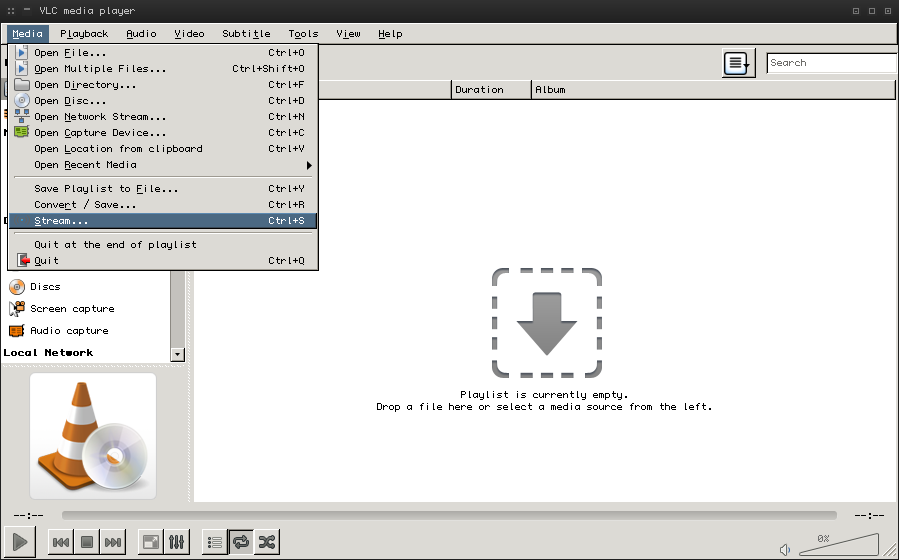
\includegraphics[width=0.9\textwidth]{1}
\end{center}

Připojte kameru (případně další záznamová zařízení) k počítači a ujistěte se že je systém dokáže detekovat. Připojte počítač k Internetu. Spusťte VLC a z nabídky {\em Media} vyberte záložku {\em Stream}\footnote{Názvy se v některých jazykových lokalizacích mohou lišit.}.


\begin{center}
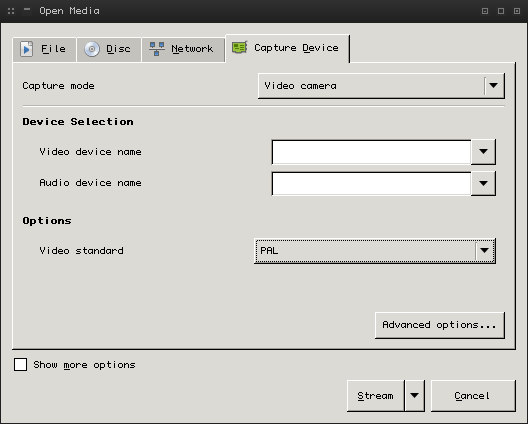
\includegraphics[width=0.9\textwidth]{3}
\end{center}

V záložce {\em Open Media} vyberte možnost {\em Capture Device} a vyberte zařízení pro záznam obrazu a zvuku z nabídky. V případě že zařízení nebylo detekováno ujistěte se že máte nainstalované patřičné ovladače pro zařízení, případně ověřte stav připojených kabelů.

Dále ze seznamu s názvem {\em Video Standart} vyberte standart odpovídající vaší připojené videokameře. Standart videa Vám zaručí jistou míru kompatibility, proto je lepší využívat tuto nabídku. Pro streaming z MiniDV kamery použijte PAL. Pro streaming z jiných kamer, speciálních zařízení, nebo zvláštních požadavků na zařízení (fixní expozice atp.) použijte {\em Advanced Options} a nastavte podrobnosti kamery manuálně.

Toto nastavení platí zatím pouze pro zařízení, ne pro samotný stream, zkuste se nastavením co nejvíce přiblížit nativnímu formátu kamery. V případě že máte méňě výkoný stroj, zde například snížením vstupního rozlišení můžete ušetřit potřebný výkon.

Po veškerém nastavení stiskněte tlačítko {\em Stream}.

\begin{center}
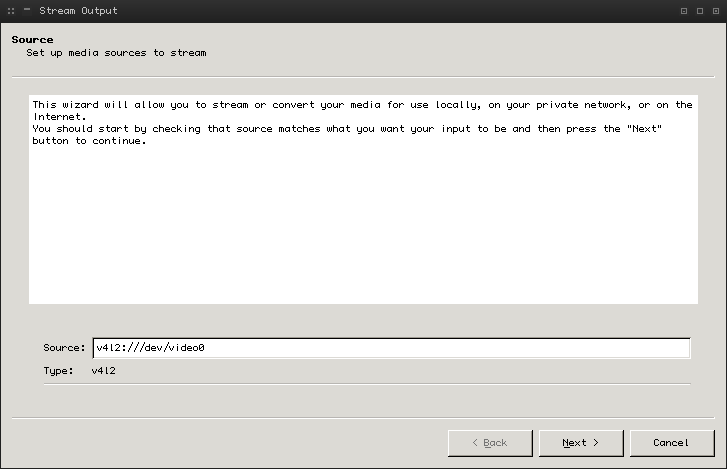
\includegraphics[width=0.9\textwidth]{4}
\end{center}

Spustí se následující průvodce, stiskněte tlačítko {\em Next}.


\begin{center}
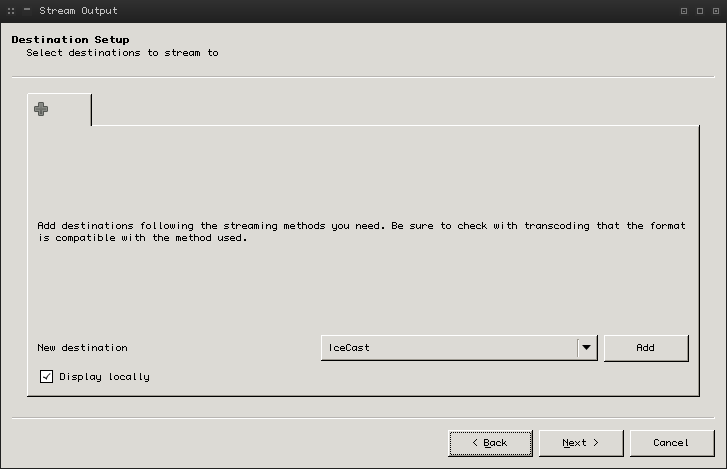
\includegraphics[width=0.9\textwidth]{5}
\end{center}

Z nabídky vyberte volbu {\em IceCast}, a nezapomeňte stisknout tlačítko {\em Add}. Zde můžete zaškrtnout i volbu {\em Display locally}, která znamená že budete mít k dispozici náhled streamu na lokálním počítači.



\begin{center}
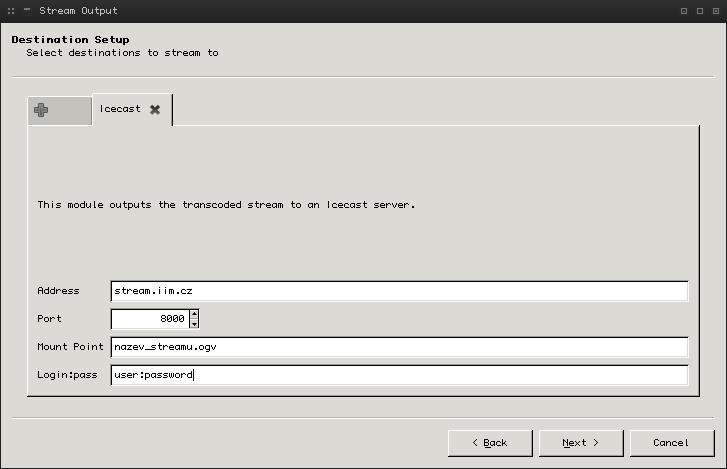
\includegraphics[width=0.9\textwidth]{6}
\end{center}

Zde vyplňte údaje o serveru. {\em Mount point} zadejte s koncovkou {\em *.ogv}. Pozor jméno uživatele a heslo jsou v jedné kolonce, odďelte tyto dva údaje dvojtečkou (bez mezer).

Stiskněte tlačítko {\em Next}.


\begin{center}
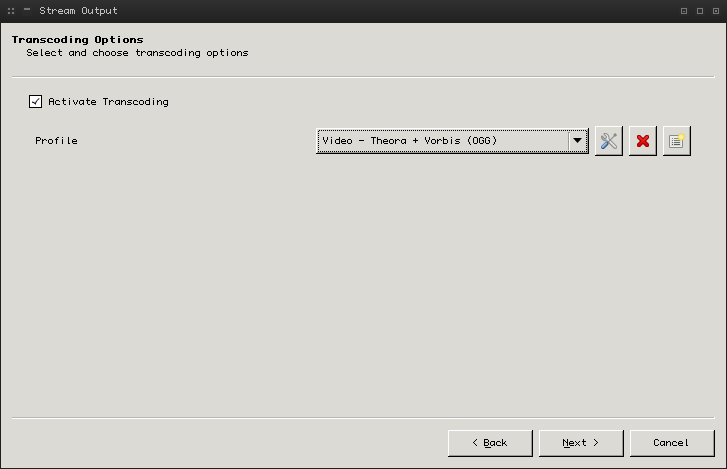
\includegraphics[width=0.9\textwidth]{7}
\end{center}

Objeví se nastavení se samotným enkódováním videa. Toto nastavení bude mít největší vliv na výslednou podobu streamu, věnujte mu tedy vyšší pozornost. Z nabídku profile vyberte variaci {\em Video - Theora + Vorbis}. V případě že taková varianta není k dispozici nainstalujte do systému patřičné kodeky.

Nyní přichází ta nejošemetnější část, nastavení rozlišení, snímků za vteřinu a bitrate streamu. Klikněte na ikonku s nářadím.


\begin{center}
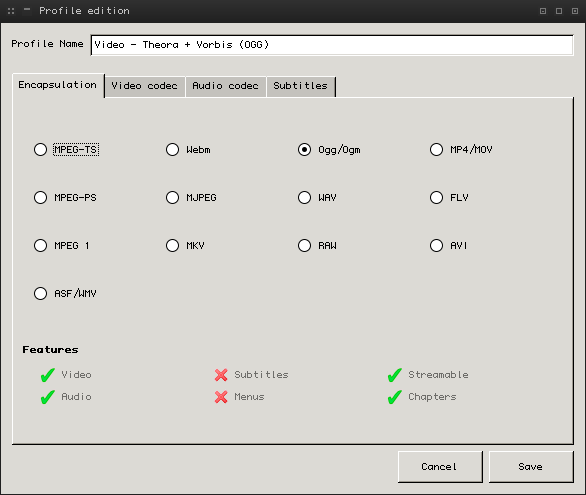
\includegraphics[width=0.9\textwidth]{8}
\end{center}

{\em Encapsluation} vyberte {\em Ogg/Ogm}


\begin{center}
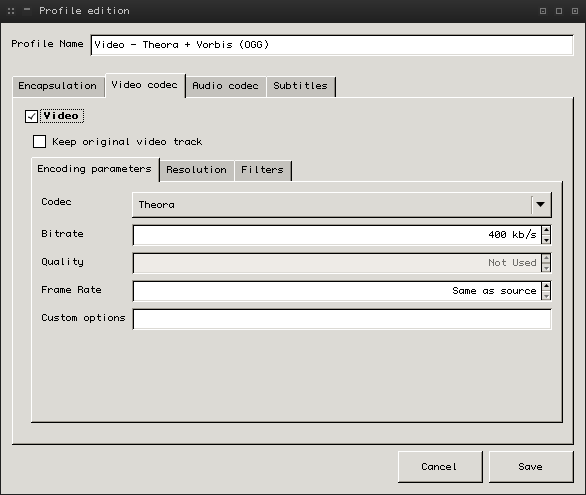
\includegraphics[width=0.9\textwidth]{9}
\end{center}

V záložce {\em Video codec} zvolte kodek {\em Theora}, v závislosti na kvalitě připojení nyní můžete upravit hodnoty pro stream. Hodnota uvedená v kb/s je cílový počet kilobitů za vteřinu. Pro ladění můžete využít jeden z online \href{http://www.bandwidthplace.com/}{testů připojení}, tyto hodnoty vám mohou vytvořit alespoň hrubou představu o řádaech rychlosti připojení a o stavu vaší sítě.\footnote{POZOR, toto je častá chyba, nikdy nezaměňte bity s bajty. Bajt = bit * 8, bity se vždy označují malým písmenem b a bajty písmenem velkým}, tedy kb/s a kB/s.

Bitrate streamu nastavujete separátně pro video a audio, přičemž výsledný datový tok bude přibližně součtem obou. Vždy si nechte alespoň čtvrtinovou rezervu (více ješte lépe) pod maximální propustnost síťě. Při testu zkuste simulovat co nejvěrněji podmínky ostrého streamu, tzn. šveknovat, zoomovat s kamerou atp. Více pohybu v obraze poměrně dramaticky zvyšuje datový tok.

Nyní můžete experimentovat, proveďte si například sérii zkoušek, pro stream vždy bude platit následující: čím větší rozlišení a počet snímků za vteřínu, tím větší datový tok, máte-li podezření na horší propustnost síťě, snižujte nejprve cílové rozlišení v záložce {\em Resolution}, ten je zde vydádřen jako násobek prvotního nastavení rozlišení kamery. Pro ucházející kvalitu obrazu, bude rychlost (400kb/s) při plném PALu (720x576 @25fps) zřejmě úplné minimum, optimální je například 1500-3000kb/s pro SD a až 4500kb/s pro HD stream. Špatnou kvalitu obrazu poznáte okamžitě, video začíná být obraz příliž ``kostičkované``, naopak moc velký datový tok bude způsobovat výpadky a zasekávání streamu. Tato fáze vyžaduje poměrně hodně trpělivosti a jistou zkušenost.


\begin{center}
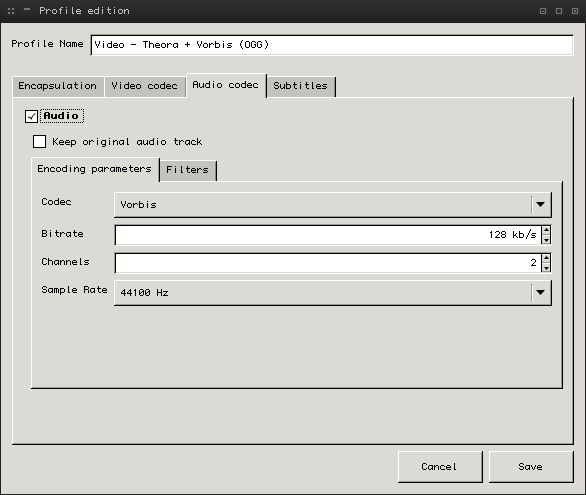
\includegraphics[width=0.9\textwidth]{10}
\end{center}

Audio kodek dále nechte na volbě Vorbis, jeho kvalitu vždy zadávejte v mocninách 2 (64,128,256kb/s), volba 128kb/s by měla být více než postačující pro přenos hlasu, vyšší volby budou vhodné pro kvalitnější hudební přenos atp.

Průvodce ukončete tlačítkem {\em save}, {\em next}.



\begin{center}
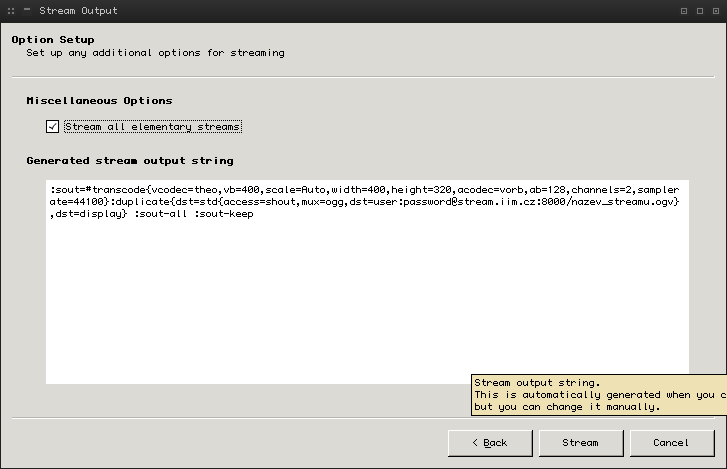
\includegraphics[width=0.9\textwidth]{11}
\end{center}

Poslední okno vám nabídne shrnutí nastavení, zaškrtněte zde pouze {\em stream all elementary streams}, talčítkem {\em stream} spustíte poprvé streaming. Nastavení si lze posléze uložit v nabídce {\em Media}, {\em Save playlist to File ...}. Stream lze dále vypínat tlačítkem stop v přehrávači a opět spouštět tlačítkem play.

\section{TODO list:}
\begin{itemize}
\item{pořízení záznamu}
\item{vhodný HW pro streaming}
\item{testovací skript na rychlost síťě, automatizace nastavení, streaming ze skriptu}
\item{streaming na lokální síti, multicast, různé typy serverů}
\end{itemize}



\section{Kontakt:}
\href{mailto:krystof.pesek@gmail.com}{krystof.pesek@gmail.com}

\end{document}
